\documentclass{beamer}
\usetheme{metropolis}

\usepackage{pgfpages}
\usepackage{xcolor}
\usepackage{pifont}
\usepackage{float}
\usepackage{minted}

%\setbeameroption{hide notes} % Only slides
%\setbeameroption{show only notes} % Only notes
\setbeameroption{show notes on second screen=right}

\title{Keep Your Laziness In Check}
\author{\textbf{Kenny Foner}, \textbf{Hengchu Zhang}, and \textbf{Leo Lampropoulos}}
\institute{University of Pennsylvania}
\date{November 20, 2017}

\definecolor{forestgreen}{rgb}{0.0, 0.75, 0.13}
\newcommand{\greentick}[0]{\color{forestgreen}\ding{51}}
\newcommand{\redcross}[0]{\color{red}\ding{55}}

\begin{document}
\frame{\titlepage}

\begin{frame}
\frametitle{Being lazy is sometimes vital, but\dots}
\Large\dots it can lead to unintended consequences.
\end{frame}

\note[itemize]{
\item Ubiquitous in Haskell programming, used in OCaml programming
\item (FRP) In the broader world, it is intrinsic in web-based functional
      reactive programming
\item (Spark) and in the field of big-data processing, for example, Spark
}

\begin{frame}[fragile]
\frametitle{Lazy lists}
\begin{minted}{ocaml}
type 'a lazyList =
  | Cons of ('a Lazy.t *
             'a lazyList Lazy.t)
  | Nil
\end{minted}
\end{frame}

\note[itemize]{
\item In this talk, we'll analyze functions that operate over lazy data structures
\item In OCaml, Lazy is a standard library module that provides operators for
      suspending computations into lazy values
\item for instance, a lazy list like this
\item A lazy list is just a list with all of its parameters wrapped in a lazy
      computation
}

\begin{frame}[fragile]
\frametitle{Lazy queues}
\begin{minted}{ocaml}
let enQ a (front,                     back) =
          (front, lazy (Cons (lazy a, back)))

let deQ (front, back) =
  match Lazy.force front with
    | Cons (a, front') -> (a, (front', back))
    | Nil ->
        let Cons (a, front') = reverseLazyList back
        in (a, (front', lazy Nil))
\end{minted}
\end{frame}

\note[itemize]{
  \item As a micro example to motivate why thinking about laziness can be
        non-trivial, let's look at this queue
  \item This has amortized O(1) performance cost.
  \item This queue is lazy as long as you don't empty the front, then it is
        fully lazy in the structure of the back list. It only forces the spine
        of the back list when the front list is emptied.
}

\iffalse
\begin{frame}
\frametitle{But it doesn't have to be this way!}
\large
Chris Okasaki:\\
``Simple and Efficient Purely Functional Queues and Deques''
\vspace{.5\baselineskip}\\
(\emph{Journal of Functional Programming}, October 1995)
\end{frame}

\note[itemize]{
\item Kenny:
\item Enqueue O(1), Dequeue O(1) NOT AMORTIZED because of laziness!
\item Guarantees valid persistently; thunks are only evaluated once
\item How do we know we have implemented the Okasaki Queues correctly?
\item Correctness != functional correctness or micro-benchmark performance:
\item == the right amount of lazy
}
\fi

\begin{frame}
\frametitle{Wouldn't it be nice to QuickCheck laziness?}
Traditional property-based testing (such as QuickCheck):
\begin{itemize}
\item[\greentick] Great for testing functional correctness
\item[\greentick] Write a specification, fuzz inputs to functions to automatically test against that specification
\item[\redcross] Can only specify and check functional correctness properties
\end{itemize}
If we were able to \textbf{specify} and \textbf{observe} laziness, we could
treat it \emph{just like} functional correctness.
\end{frame}

\note[itemize]{
\item PBRT is a technique for randomized testing which allows users to write
  down an executable specification for a function and test whether it holds for
  randomly generated inputs.
\item QuickCheck gives functional correctness
\item But laziness can't currently be observed by tools like QuickCheck
\item Laziness is not generally considered part of functional correctness much
  like how asymptotic runtime is not part of functional correctness because they
  are not directly observable
\item What if we make it observable? Then it's just part of functional correctness!
}

\begin{frame}
%\frametitle{Introducing: StrickCheck}
\Huge\centering\textbf{StrictCheck}\vspace{.15\baselineskip}\\
\Large\centering``We actually can do that thing.''
\end{frame}

\begin{frame}[fragile]
\frametitle{Observing strictness}
\begin{figure}
\centering
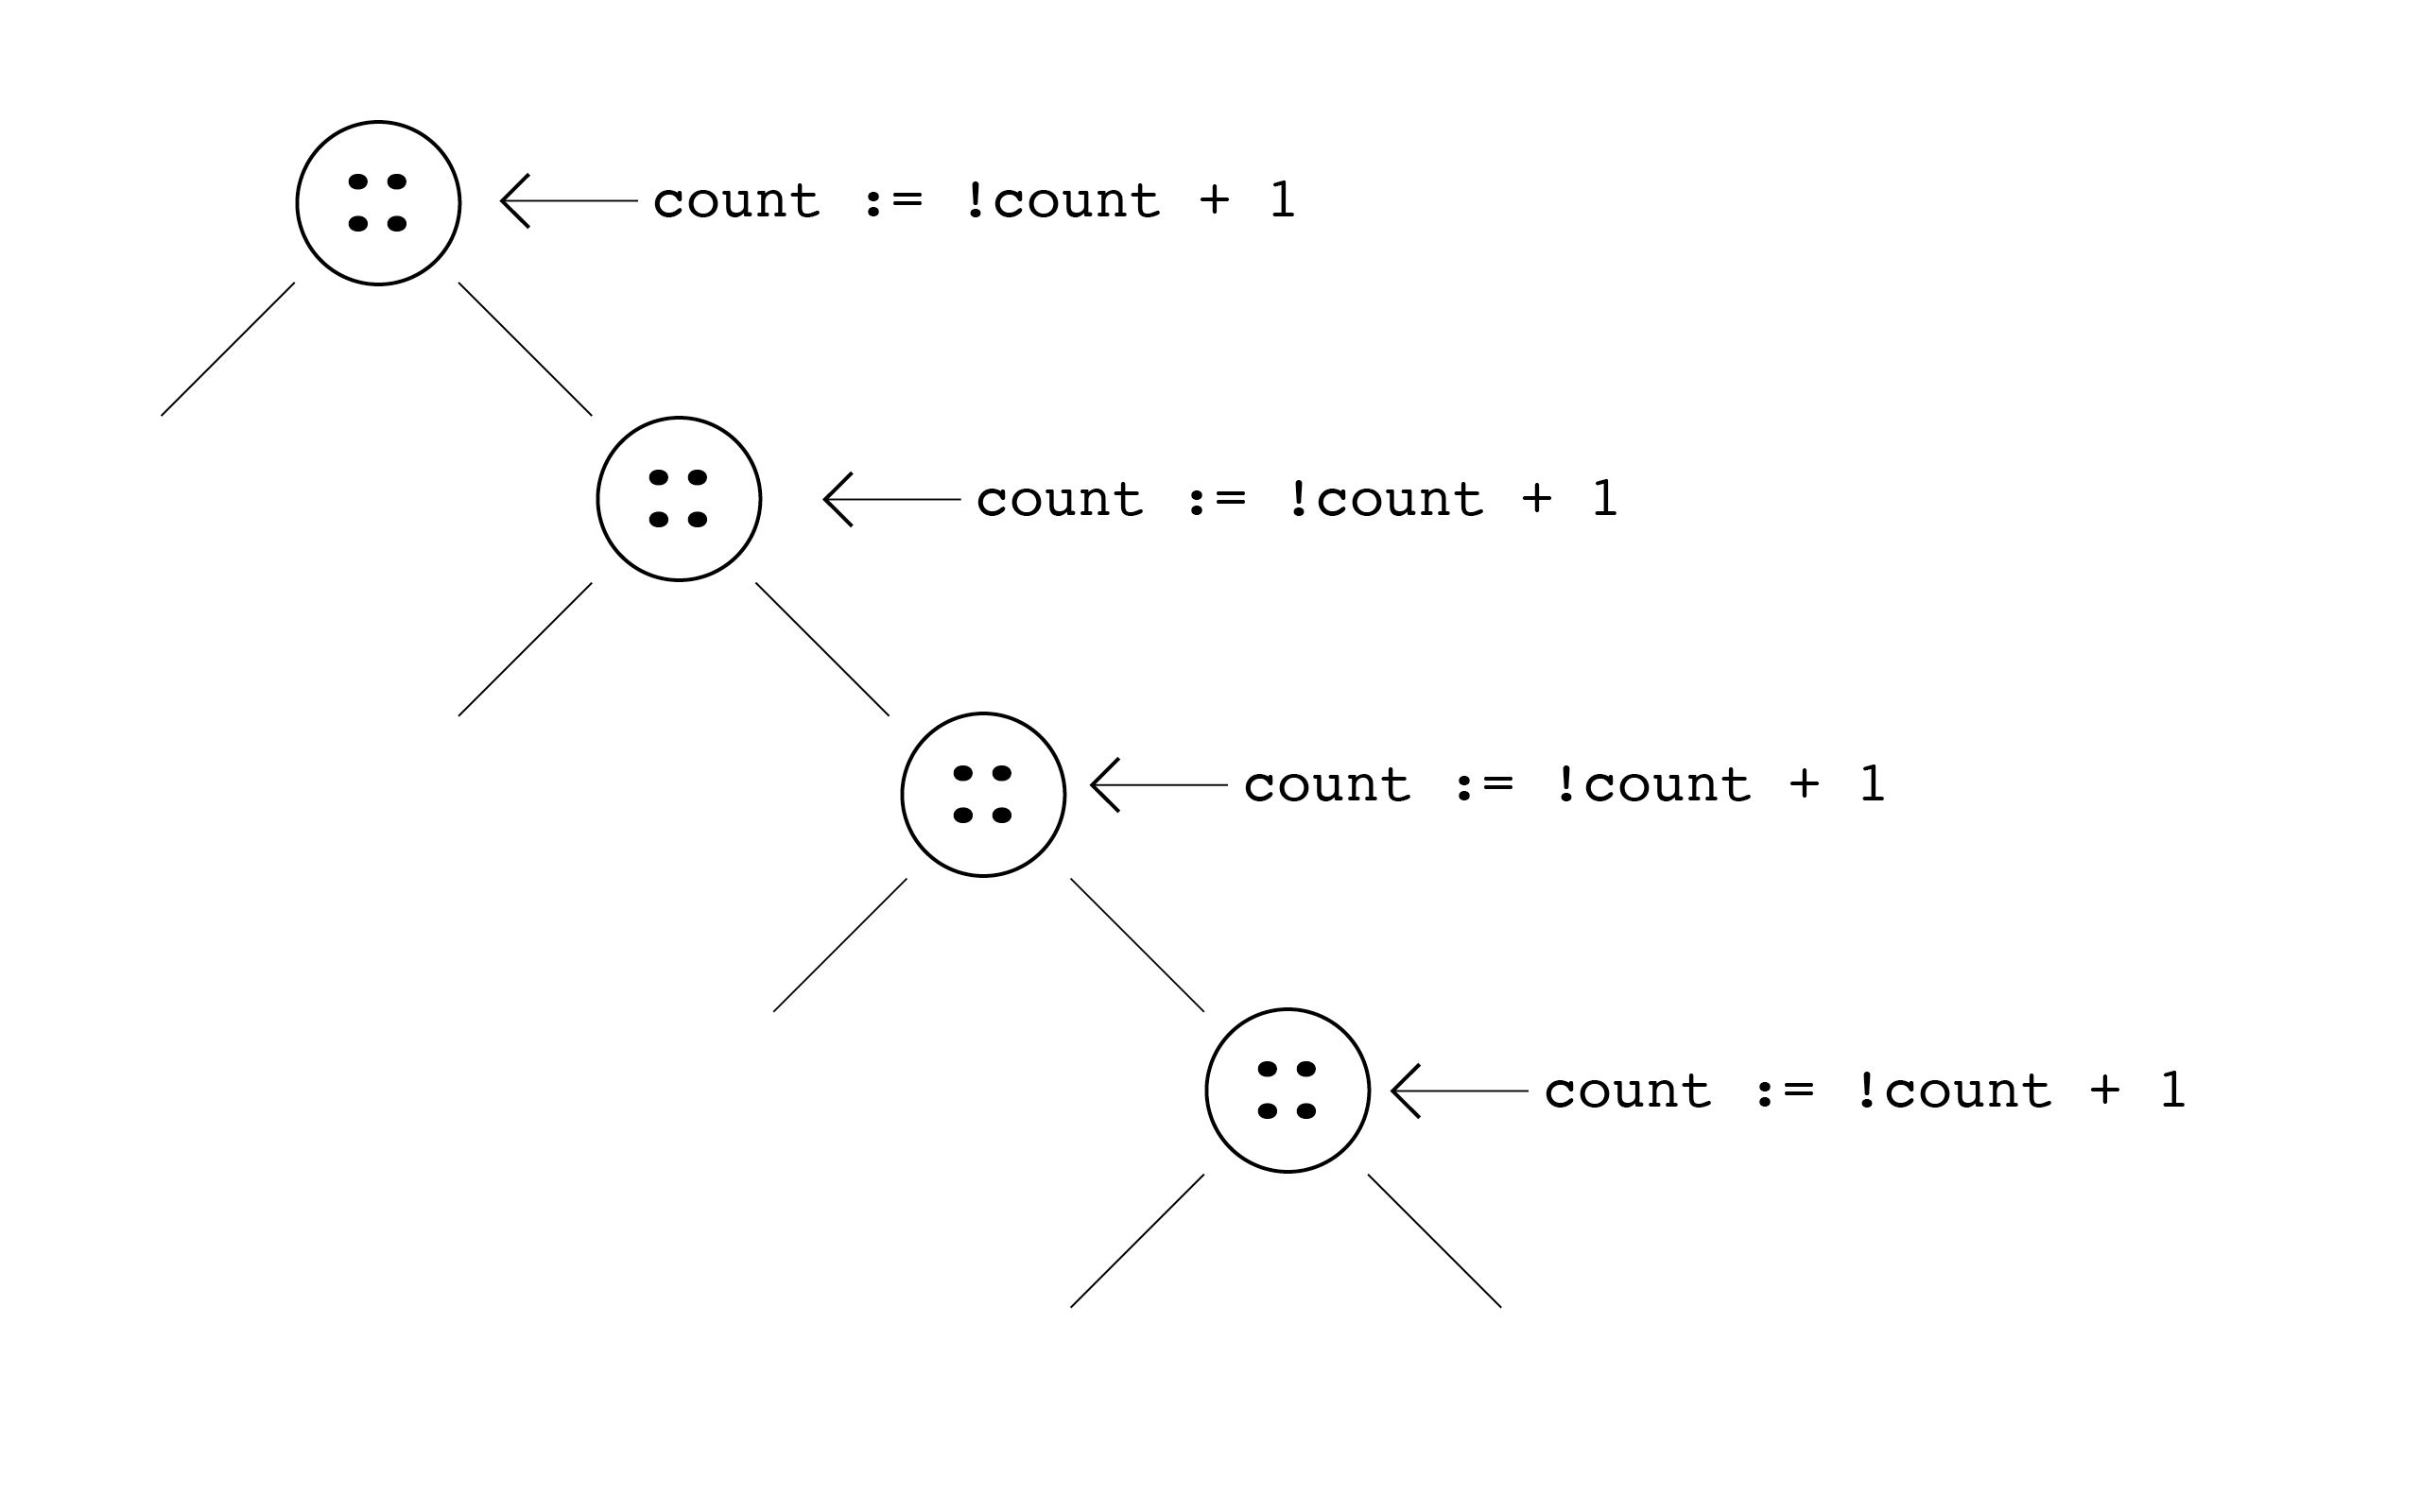
\includegraphics[width=0.6\textwidth]{instrumentListWithRef}
\caption{Instrumented List}
\end{figure}
\begin{minted}{ocaml}
instrumentListWithRef : int ref
                      -> 'a lazyList
                      -> 'a lazyList
\end{minted}
\end{frame}

\note[itemize]{
\item Hengchu:
\item \texttt{instrumentListWithRef} clones the structure of the original list,
      and attaches a lazy effectful computation to each constructor in the list.
      So as the list is evaluated, each step of evaluation triggers one update
}

\begin{frame}[fragile]
\frametitle{Strictness doesn't exist in a vacuum}
\begin{figure}
\centering
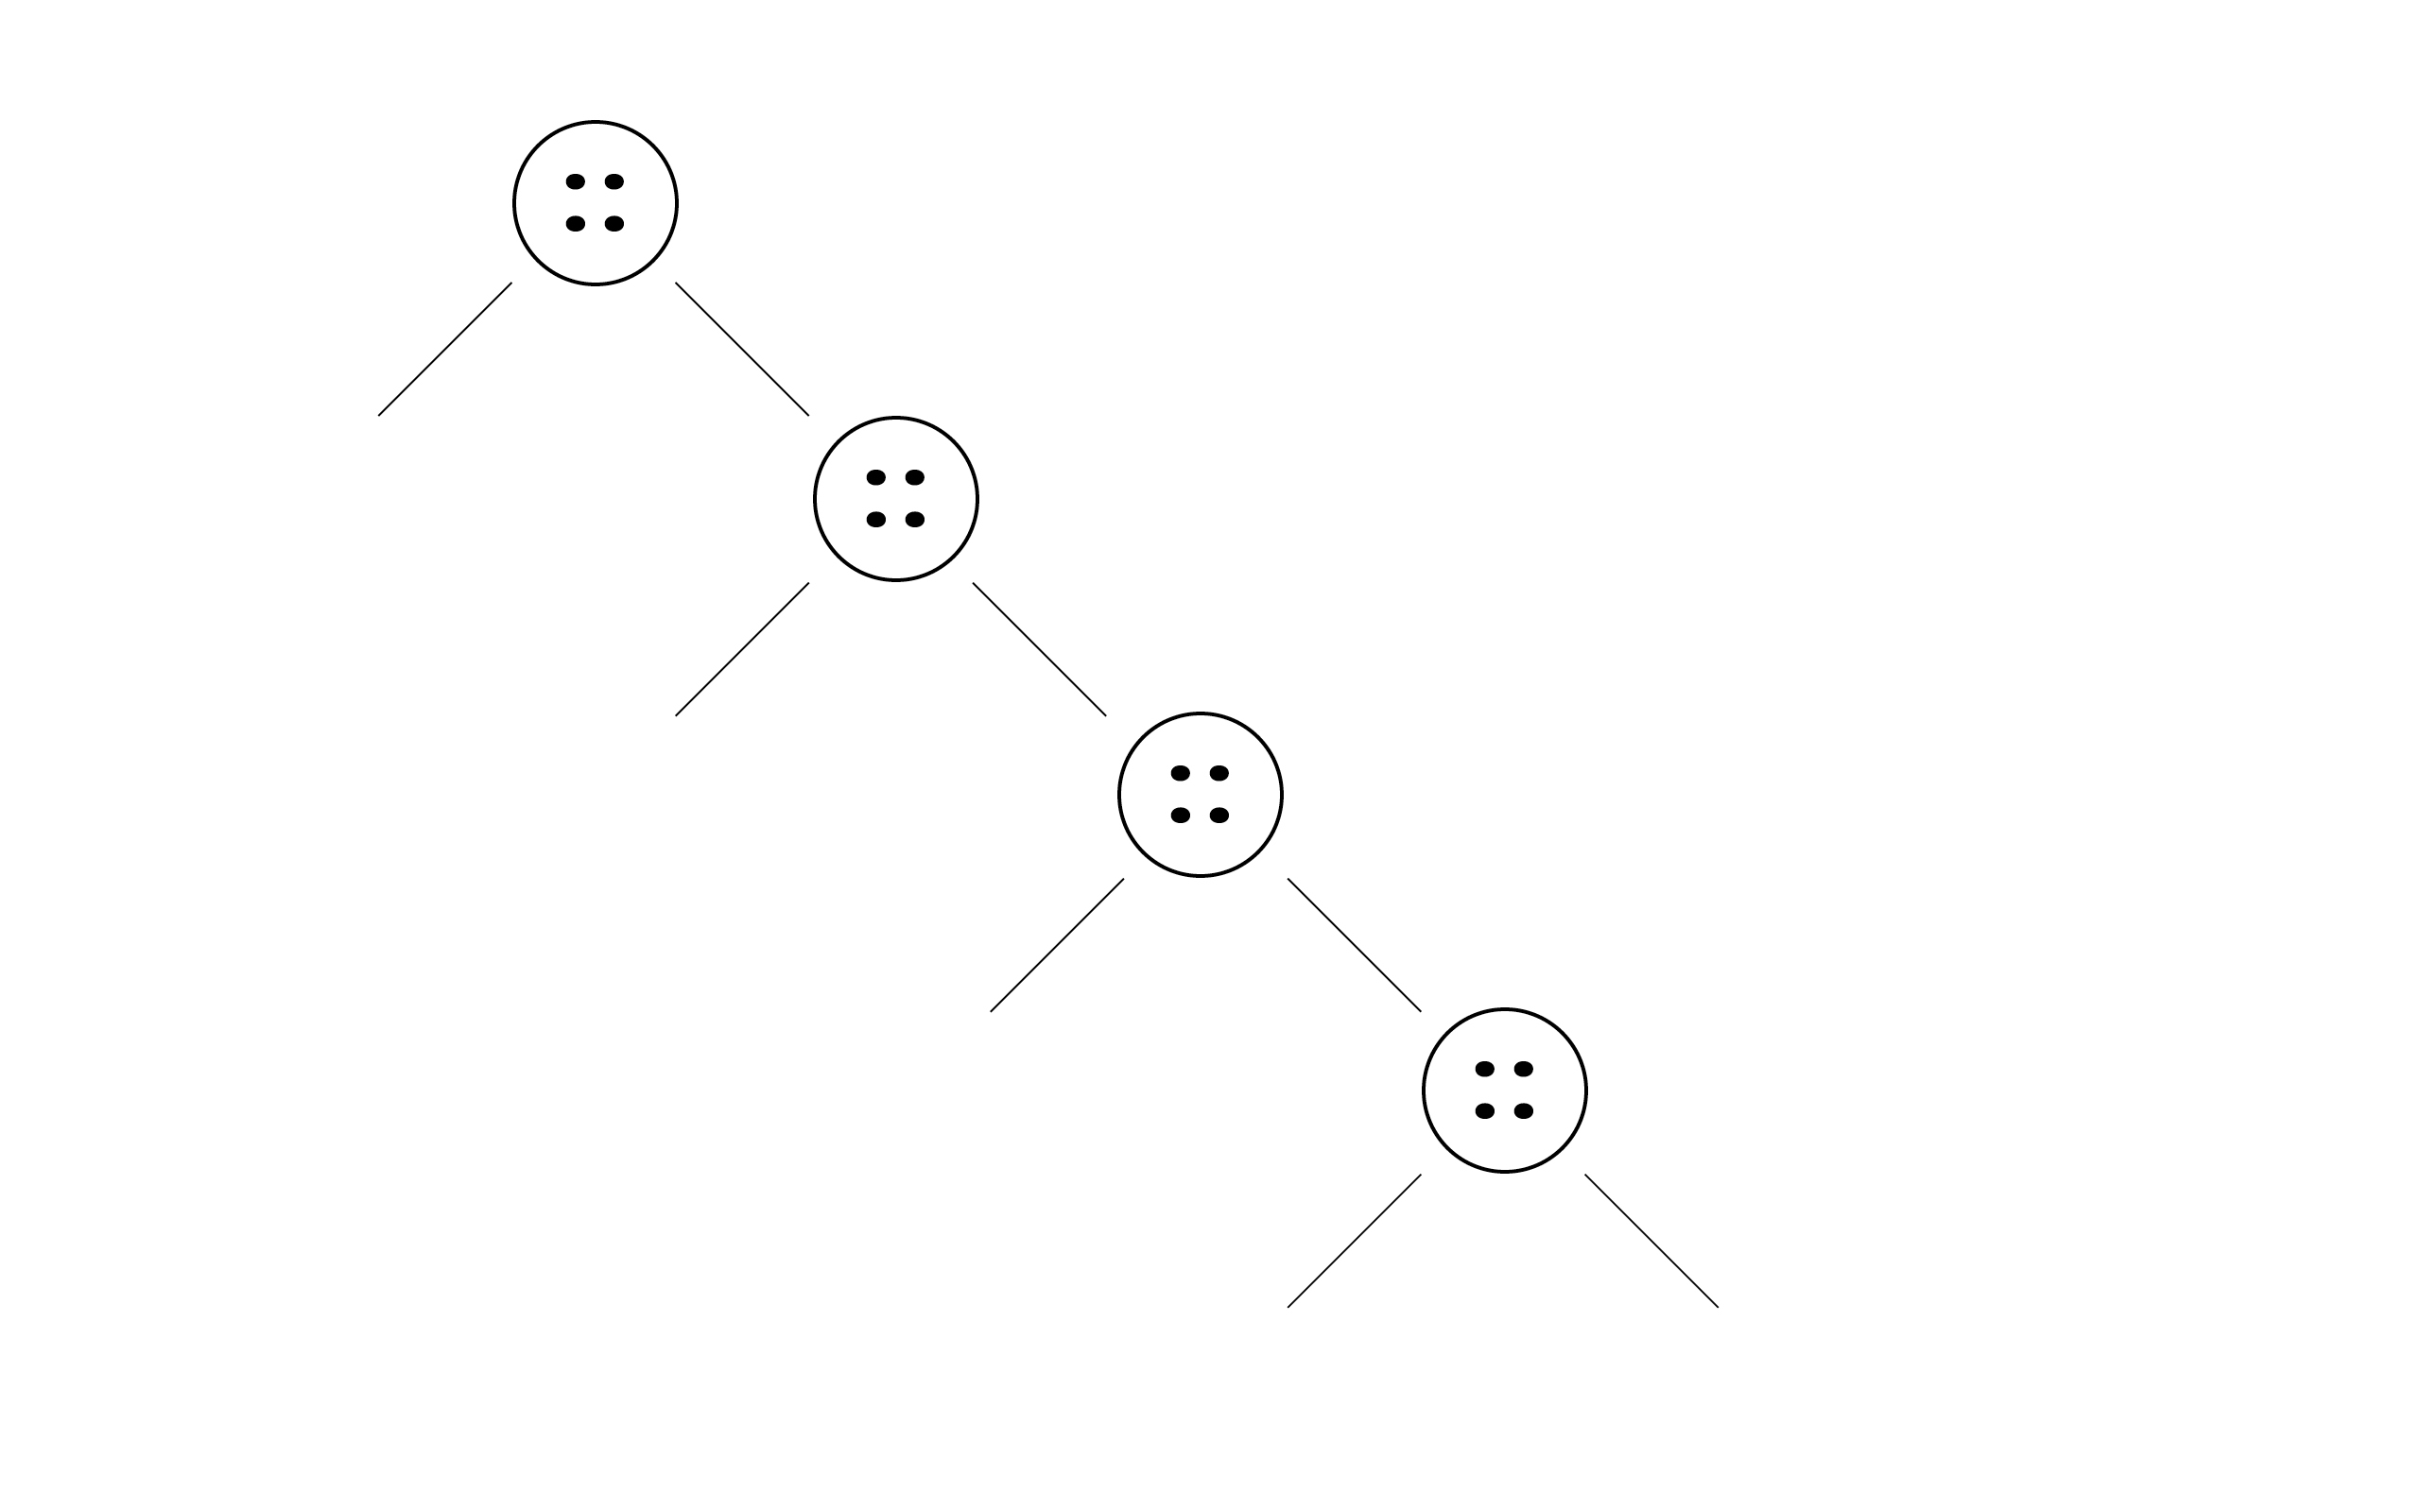
\includegraphics[width=0.7\textwidth]{noDemand}
\caption{No Demand}
\end{figure}
\end{frame}

\begin{frame}[fragile]
\frametitle{Strictness doesn't exist in a vacuum}
\begin{figure}
\centering
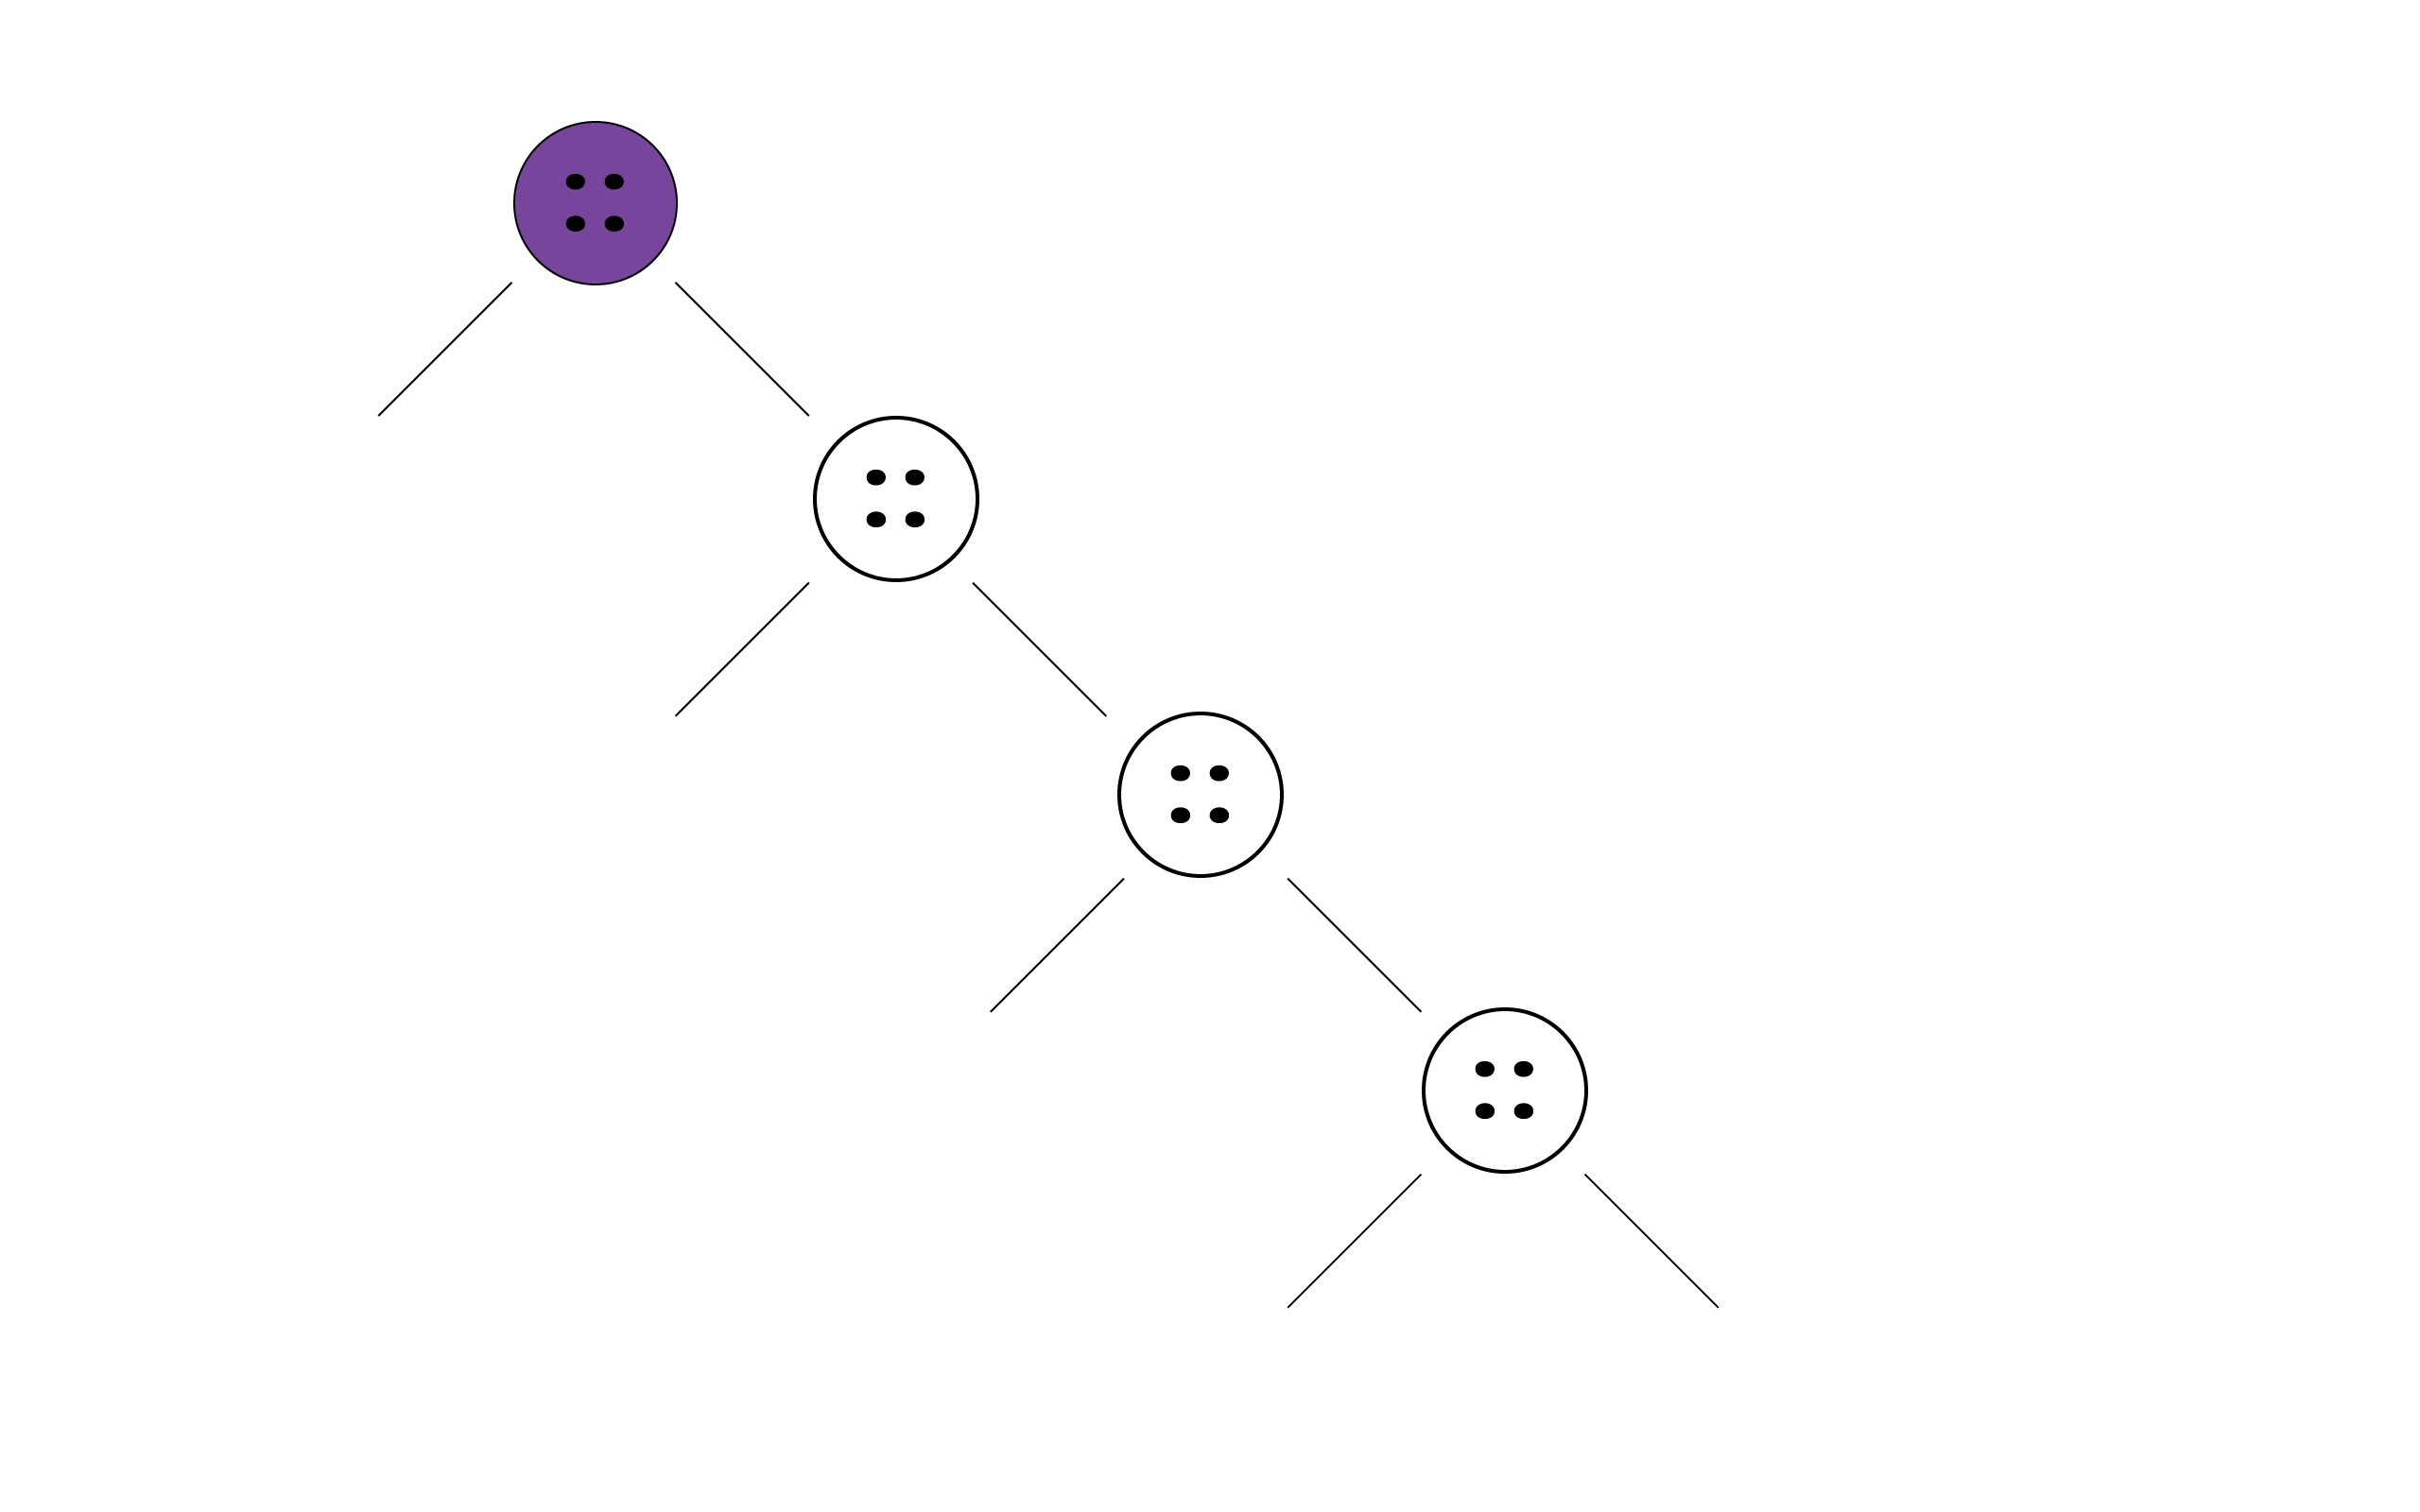
\includegraphics[width=0.7\textwidth]{whnf}
\caption{Weak Head Normal Form}
\end{figure}
\end{frame}

\begin{frame}[fragile]
\frametitle{Strictness doesn't exist in a vacuum}
\begin{figure}
\centering
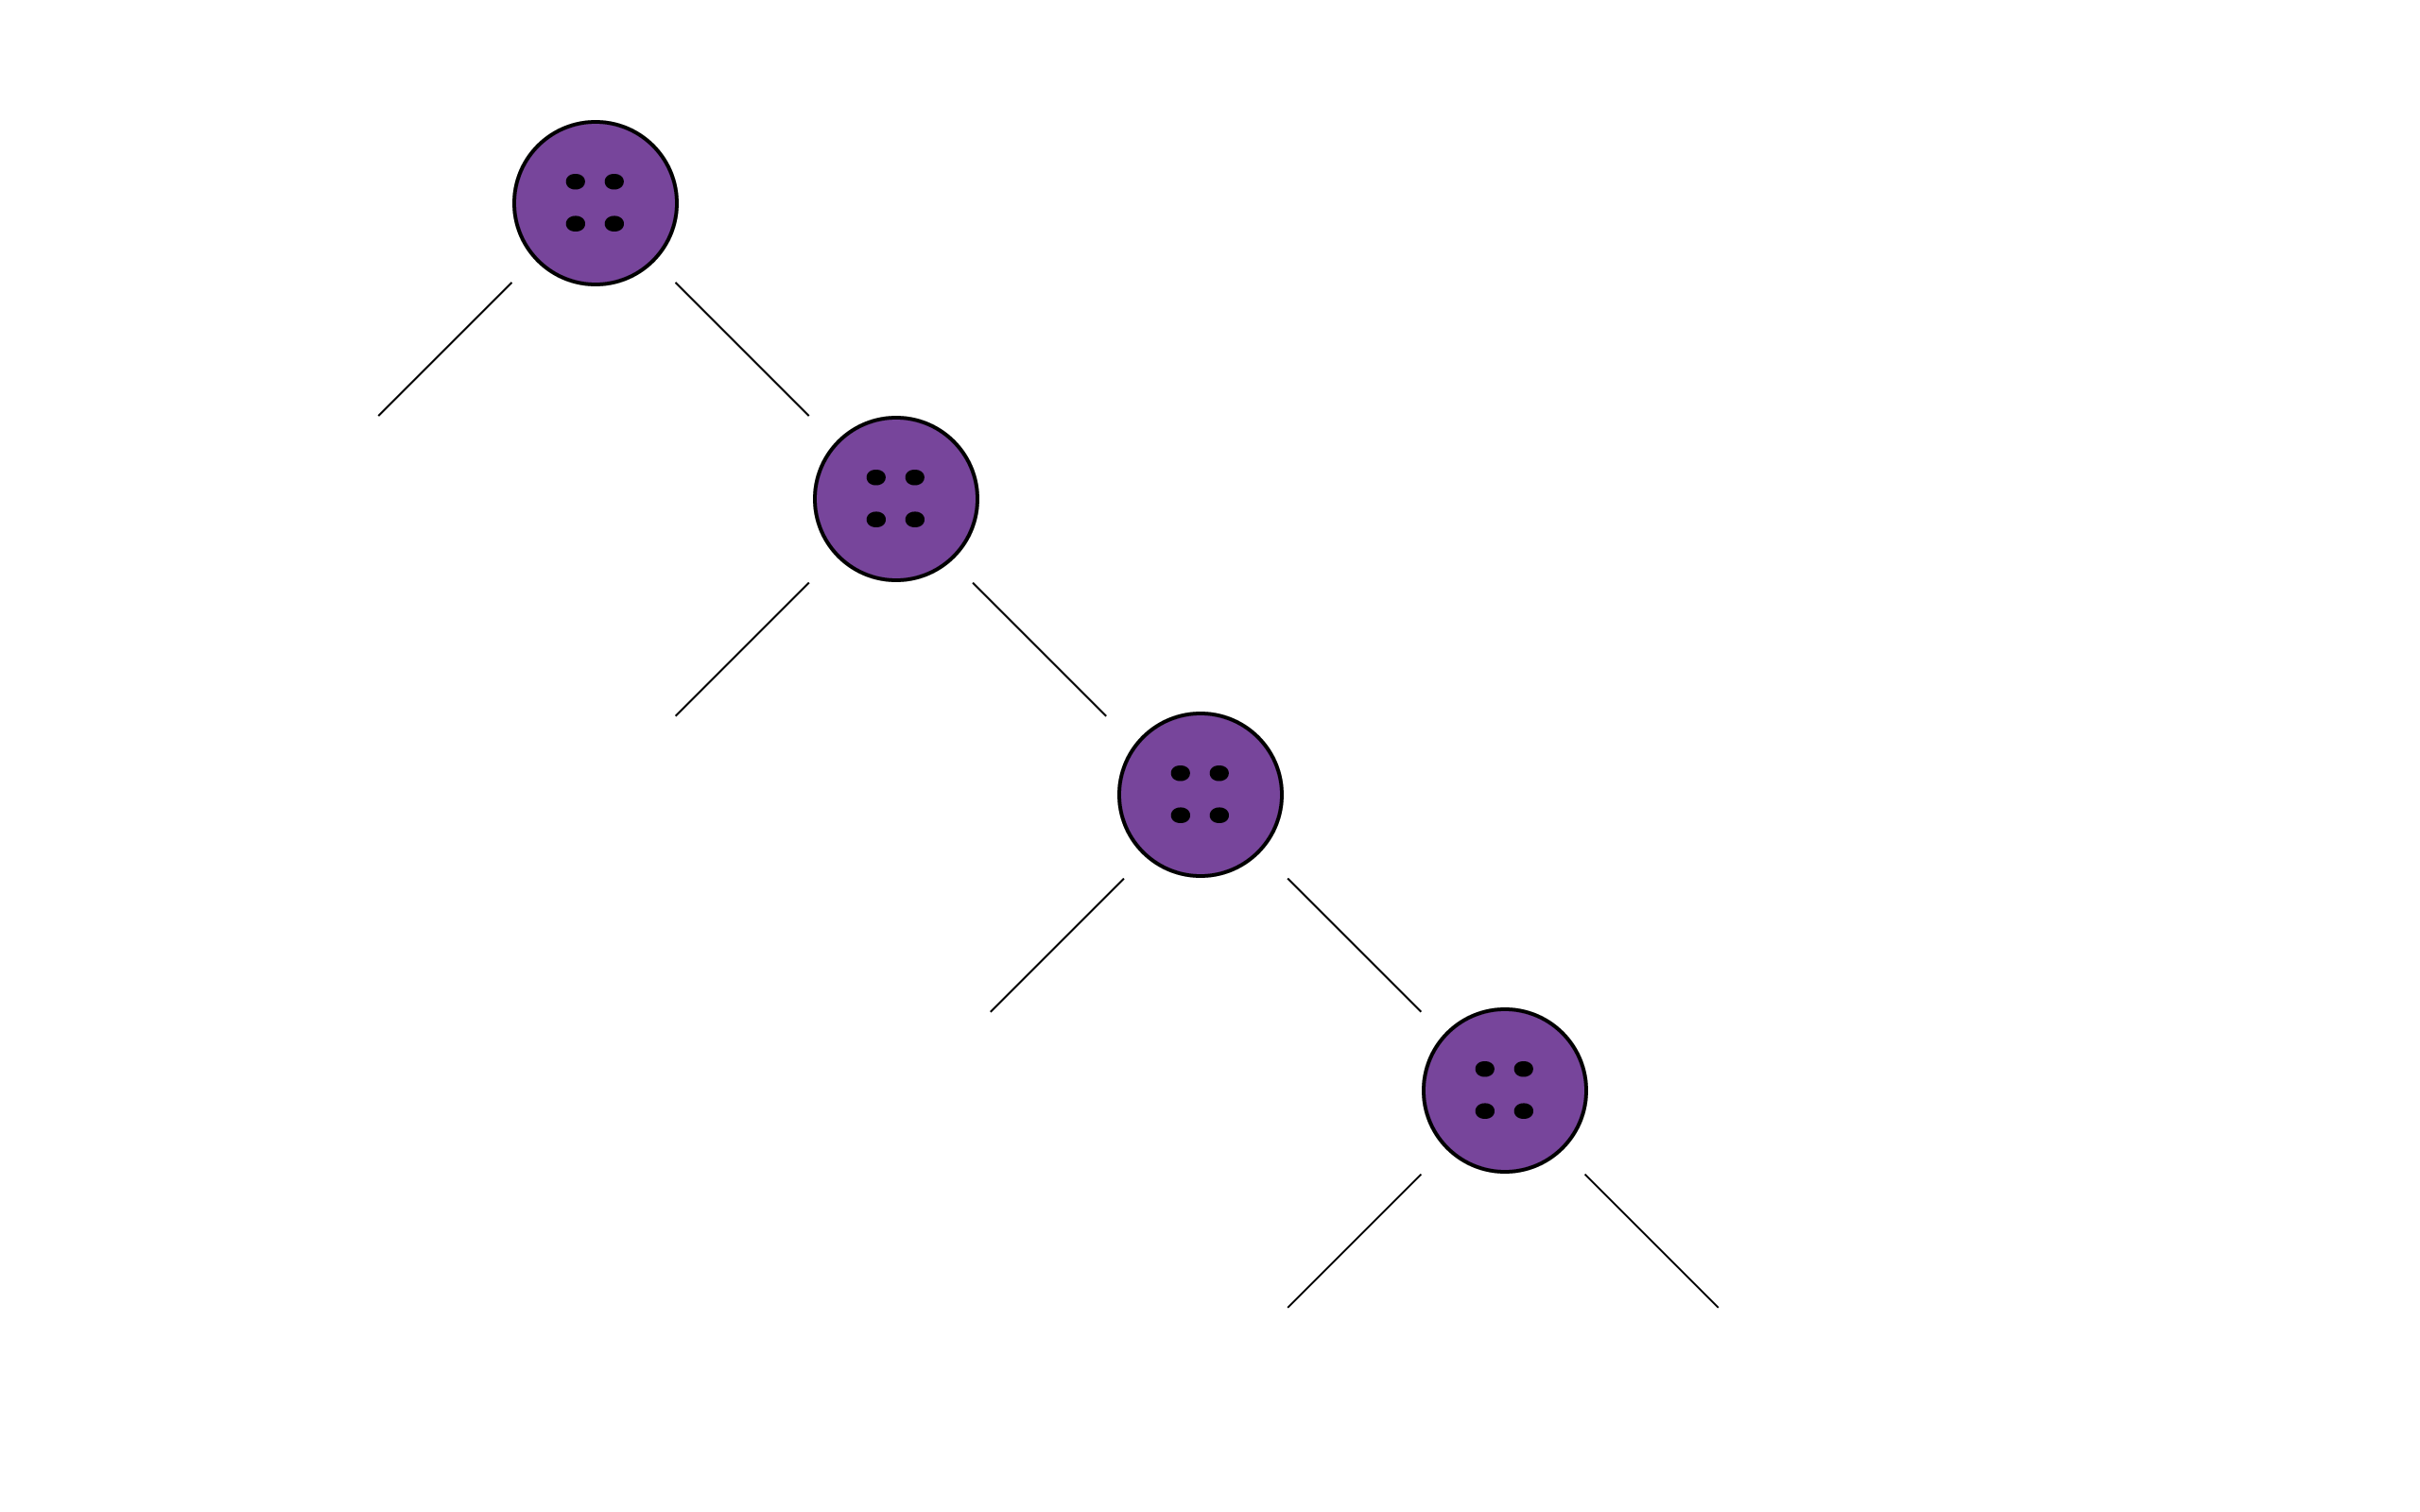
\includegraphics[width=0.7\textwidth]{spinestrict}
\caption{Spine Strict}
\end{figure}
\end{frame}

\note[itemize]{
  \item These pictures are illustrations of a demand context on a lazy list
  \item This gives us an easy way to observe the strictness behavior of a
    context
  \item While these pictures might look like a data structure, they are meant to
    describe the behavior of a context of evaluation on a lazy data structure of
    this shape }

\begin{frame}[fragile]
\frametitle{Demanding an answer, lazily}
\begin{minted}{ocaml}
demandCount context f xs =
    let count = ref 0
        observableList =
          instrumentListWithRef count xs
    in context (f observableList); !count
\end{minted}
\end{frame}

\note[itemize]{
  \item \texttt{demandCount} takes a context, and a function that operates over
        lists and the input list
  \item it applies instrumentListWithRef on the input list, producing an
        observableList, and applies the function and context over the
        observableList, triggering the injected instrumentation code
  \item context is exerting some demand on the output of f
}

\begin{frame}[fragile]
\frametitle{Examples of \texttt{demandCount}}
\begin{itemize}
\item<1->[]
\begin{verbatim}
> let f xs = takeLazy (lazy 6, xs)
> let list = toLazyList [1; 2; 3; 4; 5]
\end{verbatim}
\item<2->[]
\begin{verbatim}
> demandCount noDemand f list
\end{verbatim}
\item<3->[]
\begin{verbatim}
0
\end{verbatim}
\item<4->[]
\begin{verbatim}
> demandCount firstCons f list
\end{verbatim}
\item<5->[]
\begin{verbatim}
1
\end{verbatim}
\item<6->[]
\begin{verbatim}
> demandCount spineStrict f list
\end{verbatim}
\item<7->[]
\begin{verbatim}
5
\end{verbatim}
\end{itemize}
\end{frame}

\note[itemize]{
\item Just some examples showing demandCount
\item takeLazy is a function that takes the specified number of elements from a
      lazy list and returns a lazyList
\item Note that we simply treat \texttt{f} as a black box
\item We don't need to know anything more about \texttt{f} other than the fact
      it typechecks with demandCount!
}

\begin{frame}[fragile]
\begin{columns}
\begin{column}{0.7\textwidth}
\frametitle{Beyond lists and numbers}
\begin{figure}
\centering
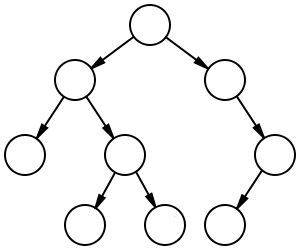
\includegraphics[width=0.7\textwidth]{binary-tree}
\end{figure}
\end{column}
\begin{column}{0.2\textwidth}
{\fontsize{100}{50}\textrm{\textbf{?}}}
\end{column}
\end{columns}
\end{frame}

\note[itemize]{
\item Kenny:
\item Arbitrary lazy algebraic datatypes
\item This gives us a bare example that counts the number of cons cells forced,
      but what if we want more fine grained information of arbitrary algebraic
      data types?
\item Numbers can't directly capture the structure of a tree, so it can't
      capture the nodes of a tree that get forced in a computation
}

\begin{frame}[fragile]
  \frametitle{Reifying demand on lazy lists}
\begin{minted}{ocaml}
type 'a lazyList =
  | Cons of ('a Lazy.t *
             'a lazyList Lazy.t)
  | Nil
------------------------------------
type 'a thunk = T | E of 'a

type 'd listDemand =
  | ConsD of ('d thunk *
              'd listDemand thunk)
  | NilD

type intDemand = IntD
\end{minted}
\end{frame}

\note[itemize]{
\item Now, we can exactly characterize a demand on a list of Ints by composing
  the type ListDemand and IntDemand
\item The type ListDemand is a reification of the demand placed upon a lazy list
  during the course of evaluation in some context }

\begin{frame}[fragile]
\frametitle{Examples}
\begin{minted}{ocaml}
type 'd listDemand =
  | ConsD of ('d thunk *
              'd listDemand thunk)
  | NilD

type intDemand = IntD
---------------------------------------------------
ConsD (T,
  ConsD (E IntD,
    ConsD (T, T)))

ConsD (E IntD,
  ConsD (T,
    ConsD (E IntD, E NilD)))
\end{minted}
\end{frame}

\note[itemize]{
  \item The 2nd Int is forced, and we force 3 cons cells, we don't force
        anything in the rest of the list
  \item The 1st and 3rd Int is forced, and the list's spine is forced
  \item Note that these represent concrete observations instrumented on given
        inputs, they do not represent the general behavior of contexts
}

\begin{frame}[fragile]
  \frametitle{Reifying demand on lazy trees}
\begin{minted}{ocaml}
type 'a lazyTree =
  | Node of ('a lazyTree Lazy.t *
             'a Lazy.t *
             'a lazyTree Lazy.t)
  | Leaf

type 'd treeDemand =
  | NodeD of ('d treeDemand thunk *
              'd thunk *
              'd treeDemand thunk)
  | LeafD
\end{minted}
\end{frame}

\note[itemize]{
  \item The demand type for a binary Tree
  \item We can either demand the value at an internal node, or one of the
        subtrees
  \item The demand type represents all of the possible prefixes/subshapes of its
        corresponding data type
}

\begin{frame}[fragile]
  \frametitle{Comparing demands on lazy lists and trees}
\begin{minted}{ocaml}
type 'd listDemand =
  | ConsD of ('d thunk *
              'd listDemand thunk)
  | NilD

type 'd treeDemand =
  | NodeD of ('d treeDemand thunk *
              'd thunk *
              'd treeDemand thunk)
  | LeafD
\end{minted}
\end{frame}

\note[itemize]{
\item Notice the similarity between ListDemand and TreeDemand with their
      corresponding data types
\item In general, the demand type of a data type simply interleaves a
      \texttt{Thunk} at every constructor field
}

\begin{frame}[fragile]
\frametitle{Observing demand, generically}
\begin{itemize}
\item<1->[]
\begin{minted}{ocaml}
demandList : 'b context -> (int lazyList -> 'b)
           -> int lazyList
           -> ('b * intDemand listDemand thunk)

demandTree : 'b context -> (int lazyTree -> 'b)
           -> int lazyTree
           -> ('b * intDemand treeDemand thunk)
\end{minted}
\item<2->[]
\begin{minted}{ocaml}
------------------------------------------------
demand     : 'b context -> ('a -> 'b) -> 'a
           -> ('b * ('a DEMAND) thunk)
\end{minted}
\end{itemize}
\end{frame}

\note[itemize]{
\item There is a determinate relation between a lazy data structure and its
      demand representation
\item We return a \texttt{Thunk} of demand because the input might not be
      demanded at all
\item We expect that the 'a parameter is some kind of lazy structure, and 'b is
      also some kind of lazy structure
\item We use generic programming to implement the DEMAND type for all algebraic
      data types
}

\iffalse
\begin{frame}[fragile]
\frametitle{Generic \texttt{Demand} calculation}
\begin{minted}{haskell}
type family Demand (x :: *) :: * where
 Demand (a -> b)  = FuncDemand
 Demand (a :+: b) = Demand a :+: Demand b
 Demand (a :*: b) = Thunk (Demand a) :*: Thunk (Demand b)
\end{minted}
\end{frame}

\note[itemize]{
\item For simplicity, we speak of types in terms of sums and products
\item \texttt{FuncDemand} is isomorphic to IntDemand in that it only captures
  whether the function was used at all } \fi

\begin{frame}[fragile]
  \frametitle{Recalling \texttt{deQ}}
  \begin{minted}{ocaml}
type 'a lazyList =
  | Cons of ('a Lazy.t *
             'a lazyList Lazy.t)
  | Nil

let deQ (front, back)
  : ('a Lazy.t * ('a lazyList Lazy.t *
                  'a lazyList Lazy.t)) =
  match Lazy.force front with
    | Cons (a, front') -> (a, (front', back))
    | Nil ->
        let Cons (a, front') = reverseLazyList back
        in (a, (front', lazy Nil))
  \end{minted}
\end{frame}

\begin{frame}[fragile]
\frametitle{First-order specifications}
\begin{minted}{ocaml}
let spec_deQ (front, back) (dInt, (dFront, dBack)) =
  match Lazy.force front with
    | Cons (_, _) ->
        (E (ConsD (dInt, dFront)), dBack)
    | Nil -> (E NilD,
              spineStrictAs back
                (pad (length back - lengthD dFront)
                     (reverseD (ConsD dInt dFront))))
\end{minted}
\end{frame}

\note[itemize]{
  \item Having demonstrated how to reify demand behaviors into value, we now
        need to figure out how to write down a specification to check if whether
        a particular run of the program has the specified laziness according to
        the specification
  \item Specifications go backwards from demands on the output to demands on
        the inputs of the function. This is because how much input is demanded
        depends on how much output is demanded, hence the arrows go the other
        way.
  \item Specifications are passed in the actual values of the inputs because
        their demand behaviors can be dependent on those inputs
  \item spineStrictAs takes a lazy data structure, and unions a spine strict
        demand corresponding to the whole structure with another demand on some
        sub-part of that structure
}

\begin{frame}[fragile]
\frametitle{Connecting specification with observation}
\begin{figure}
\centering
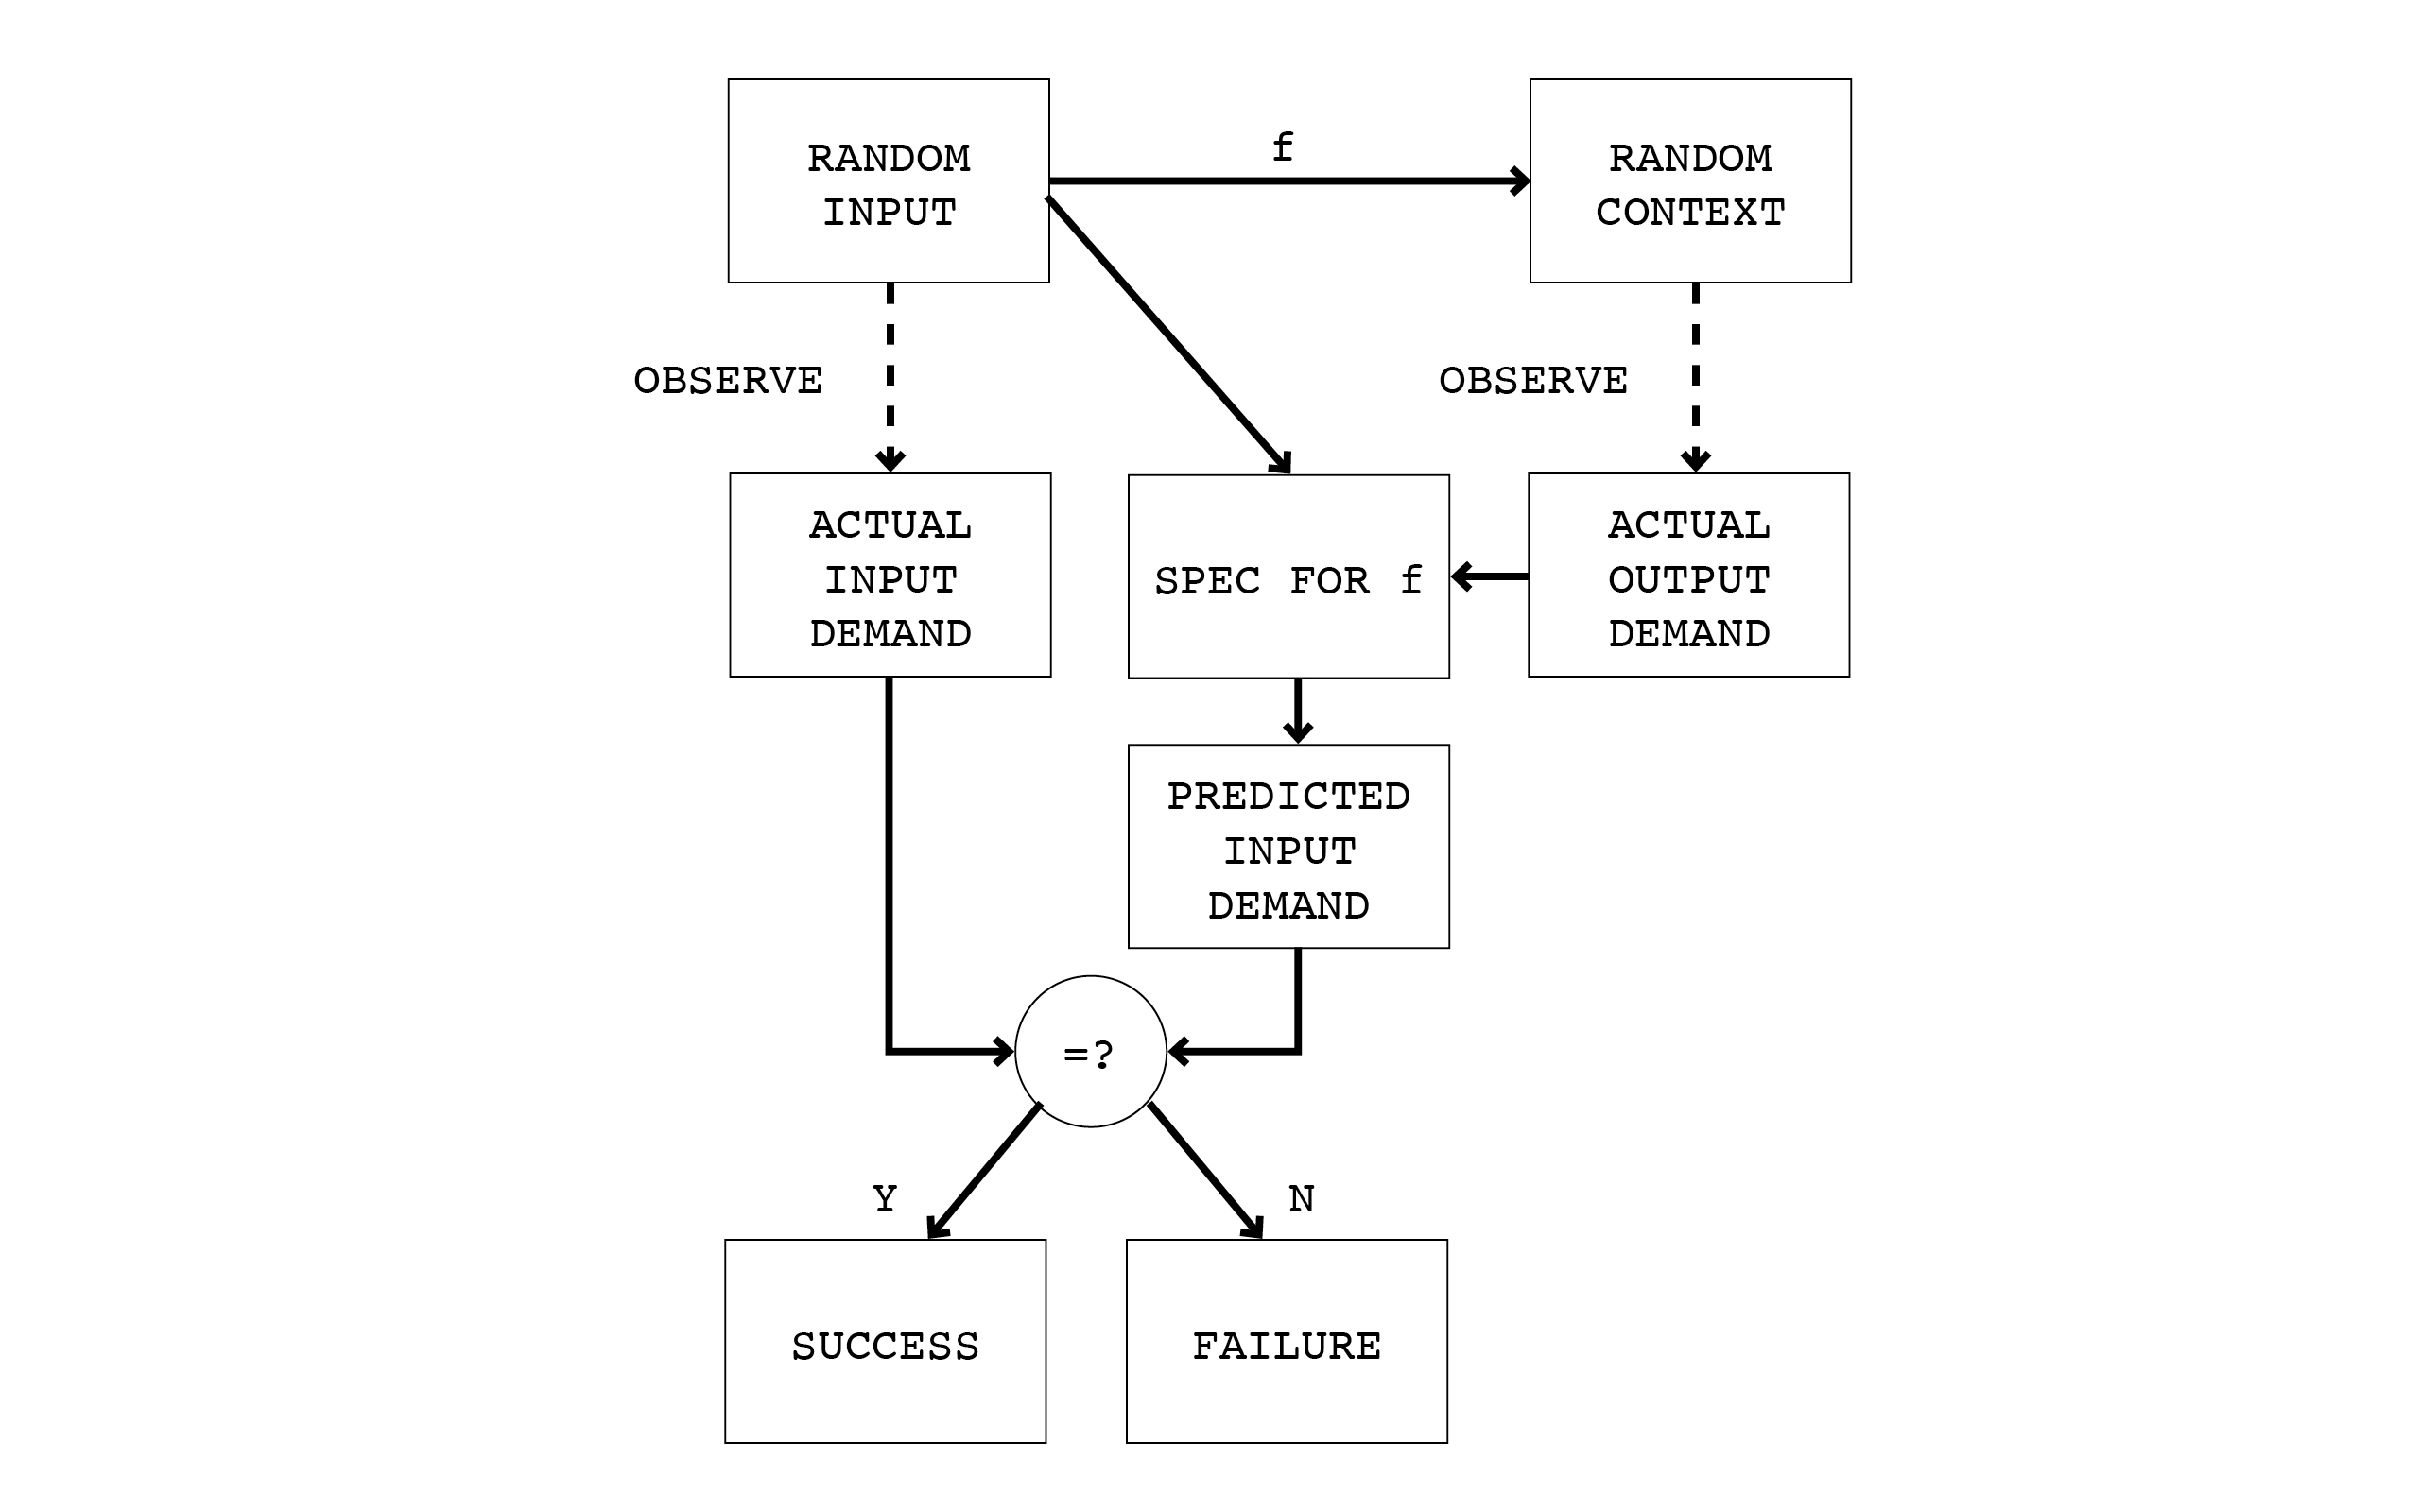
\includegraphics[width=1.0\textwidth]{specflow}
\end{figure}
\end{frame}

\note[itemize]{
\item We randomly fuzz the inputs to the function, and
  \item We can generate random contexts
        that exert non-trivial demand on the output values
  \item We observe the demand on the input and also the demand on the
        output, so we can just straightforwardly compare that to what
        the specification expects.
}

\iffalse
\begin{frame}[fragile]
\frametitle{Higher-order specifications}
\end{frame}

\note[itemize]{
  \item There is in fact also a mechanical transformation between the type of a
        function to the type of its demand specification
  \item Moreover, this transformation works even with high-order functions
  \item Higher-order specifications will take specification of their input
        functions because their demand behavior is parameterized over the demand
        behavior of their input functions
  \item At testing time, these specifications can be fuzzed through the same
        \texttt{CoArbitrary} mechanism
}
\fi

\begin{frame}[fragile]
\frametitle{Contributions}
With \textbf{StrictCheck}, you will be able to:
\begin{itemize}
\item \textbf{Observe} laziness from within Haskell
\item \textbf{Specify} laziness properties as Haskell functions
\item \textbf{Test} implementations against those specifications
\item \textbf{For all types},\footnotemark\, including higher-order functions and
      data types containing functions
\end{itemize}
The implementation is a work in progress.
\footnotetext[1]{Simple (i.e. non-indexed, non-existential) types}
\end{frame}

\begin{frame}[fragile]
\frametitle{Have questions?}
Ask us about \dots
\begin{itemize}
\item Higher-order specifications
\item Generic programming for any arity and datatype
\item Random generation of partial demand contexts
\item Shrinking of contexts and inputs
\item Efficiency of our implementation
\item Details of instrumentation
\item What language are you actually implementing this in? \\ (Hint: it's not ML)
\item[] \ \ $\vdots$
\end{itemize}
\end{frame}


\end{document}
